\PassOptionsToPackage{unicode=true}{hyperref} % options for packages loaded elsewhere
\PassOptionsToPackage{hyphens}{url}
%
\documentclass[]{article}
\usepackage{lmodern}
\usepackage{amssymb,amsmath}
\usepackage{ifxetex,ifluatex}
\usepackage{fixltx2e} % provides \textsubscript
\ifnum 0\ifxetex 1\fi\ifluatex 1\fi=0 % if pdftex
  \usepackage[T1]{fontenc}
  \usepackage[utf8]{inputenc}
  \usepackage{textcomp} % provides euro and other symbols
\else % if luatex or xelatex
  \usepackage{unicode-math}
  \defaultfontfeatures{Ligatures=TeX,Scale=MatchLowercase}
\fi
% use upquote if available, for straight quotes in verbatim environments
\IfFileExists{upquote.sty}{\usepackage{upquote}}{}
% use microtype if available
\IfFileExists{microtype.sty}{%
\usepackage[]{microtype}
\UseMicrotypeSet[protrusion]{basicmath} % disable protrusion for tt fonts
}{}
\IfFileExists{parskip.sty}{%
\usepackage{parskip}
}{% else
\setlength{\parindent}{0pt}
\setlength{\parskip}{6pt plus 2pt minus 1pt}
}
\usepackage{hyperref}
\hypersetup{
            pdftitle={103hw5},
            pdfborder={0 0 0},
            breaklinks=true}
\urlstyle{same}  % don't use monospace font for urls
\usepackage[margin=1in]{geometry}
\usepackage{color}
\usepackage{fancyvrb}
\newcommand{\VerbBar}{|}
\newcommand{\VERB}{\Verb[commandchars=\\\{\}]}
\DefineVerbatimEnvironment{Highlighting}{Verbatim}{commandchars=\\\{\}}
% Add ',fontsize=\small' for more characters per line
\usepackage{framed}
\definecolor{shadecolor}{RGB}{248,248,248}
\newenvironment{Shaded}{\begin{snugshade}}{\end{snugshade}}
\newcommand{\AlertTok}[1]{\textcolor[rgb]{0.94,0.16,0.16}{#1}}
\newcommand{\AnnotationTok}[1]{\textcolor[rgb]{0.56,0.35,0.01}{\textbf{\textit{#1}}}}
\newcommand{\AttributeTok}[1]{\textcolor[rgb]{0.77,0.63,0.00}{#1}}
\newcommand{\BaseNTok}[1]{\textcolor[rgb]{0.00,0.00,0.81}{#1}}
\newcommand{\BuiltInTok}[1]{#1}
\newcommand{\CharTok}[1]{\textcolor[rgb]{0.31,0.60,0.02}{#1}}
\newcommand{\CommentTok}[1]{\textcolor[rgb]{0.56,0.35,0.01}{\textit{#1}}}
\newcommand{\CommentVarTok}[1]{\textcolor[rgb]{0.56,0.35,0.01}{\textbf{\textit{#1}}}}
\newcommand{\ConstantTok}[1]{\textcolor[rgb]{0.00,0.00,0.00}{#1}}
\newcommand{\ControlFlowTok}[1]{\textcolor[rgb]{0.13,0.29,0.53}{\textbf{#1}}}
\newcommand{\DataTypeTok}[1]{\textcolor[rgb]{0.13,0.29,0.53}{#1}}
\newcommand{\DecValTok}[1]{\textcolor[rgb]{0.00,0.00,0.81}{#1}}
\newcommand{\DocumentationTok}[1]{\textcolor[rgb]{0.56,0.35,0.01}{\textbf{\textit{#1}}}}
\newcommand{\ErrorTok}[1]{\textcolor[rgb]{0.64,0.00,0.00}{\textbf{#1}}}
\newcommand{\ExtensionTok}[1]{#1}
\newcommand{\FloatTok}[1]{\textcolor[rgb]{0.00,0.00,0.81}{#1}}
\newcommand{\FunctionTok}[1]{\textcolor[rgb]{0.00,0.00,0.00}{#1}}
\newcommand{\ImportTok}[1]{#1}
\newcommand{\InformationTok}[1]{\textcolor[rgb]{0.56,0.35,0.01}{\textbf{\textit{#1}}}}
\newcommand{\KeywordTok}[1]{\textcolor[rgb]{0.13,0.29,0.53}{\textbf{#1}}}
\newcommand{\NormalTok}[1]{#1}
\newcommand{\OperatorTok}[1]{\textcolor[rgb]{0.81,0.36,0.00}{\textbf{#1}}}
\newcommand{\OtherTok}[1]{\textcolor[rgb]{0.56,0.35,0.01}{#1}}
\newcommand{\PreprocessorTok}[1]{\textcolor[rgb]{0.56,0.35,0.01}{\textit{#1}}}
\newcommand{\RegionMarkerTok}[1]{#1}
\newcommand{\SpecialCharTok}[1]{\textcolor[rgb]{0.00,0.00,0.00}{#1}}
\newcommand{\SpecialStringTok}[1]{\textcolor[rgb]{0.31,0.60,0.02}{#1}}
\newcommand{\StringTok}[1]{\textcolor[rgb]{0.31,0.60,0.02}{#1}}
\newcommand{\VariableTok}[1]{\textcolor[rgb]{0.00,0.00,0.00}{#1}}
\newcommand{\VerbatimStringTok}[1]{\textcolor[rgb]{0.31,0.60,0.02}{#1}}
\newcommand{\WarningTok}[1]{\textcolor[rgb]{0.56,0.35,0.01}{\textbf{\textit{#1}}}}
\usepackage{graphicx,grffile}
\makeatletter
\def\maxwidth{\ifdim\Gin@nat@width>\linewidth\linewidth\else\Gin@nat@width\fi}
\def\maxheight{\ifdim\Gin@nat@height>\textheight\textheight\else\Gin@nat@height\fi}
\makeatother
% Scale images if necessary, so that they will not overflow the page
% margins by default, and it is still possible to overwrite the defaults
% using explicit options in \includegraphics[width, height, ...]{}
\setkeys{Gin}{width=\maxwidth,height=\maxheight,keepaspectratio}
\setlength{\emergencystretch}{3em}  % prevent overfull lines
\providecommand{\tightlist}{%
  \setlength{\itemsep}{0pt}\setlength{\parskip}{0pt}}
\setcounter{secnumdepth}{0}
% Redefines (sub)paragraphs to behave more like sections
\ifx\paragraph\undefined\else
\let\oldparagraph\paragraph
\renewcommand{\paragraph}[1]{\oldparagraph{#1}\mbox{}}
\fi
\ifx\subparagraph\undefined\else
\let\oldsubparagraph\subparagraph
\renewcommand{\subparagraph}[1]{\oldsubparagraph{#1}\mbox{}}
\fi

% set default figure placement to htbp
\makeatletter
\def\fps@figure{htbp}
\makeatother


\title{103hw5}
\author{}
\date{\vspace{-2.5em}}

\begin{document}
\maketitle

\begin{center}\rule{0.5\linewidth}{0.5pt}\end{center}

\begin{enumerate}
\def\labelenumi{\arabic{enumi}.}
\tightlist
\item
  Construct a simple linear regression model for Highway MPG vs
  Horsepower.
\end{enumerate}

\begin{enumerate}
\def\labelenumi{\alph{enumi}.}
\tightlist
\item
  Is the P-value for the model significant? (Quote the P-value in your
  response.) yes the P-value is 3.7e-11 \textless{} .05 so it is
  significant.
\item
  What is R2 for the model? R2 is .3832
\item
  Graph the Plot of Fitted Model and include it in your solutions. Use
  it to describe the problem with the model. ***
\end{enumerate}

\begin{Shaded}
\begin{Highlighting}[]
\KeywordTok{library}\NormalTok{(readxl)}
\NormalTok{cars <-}\StringTok{ }\KeywordTok{read_excel}\NormalTok{(}\StringTok{"/Users/austinwilson/downloads/93cars.xlsx"}\NormalTok{)}
\NormalTok{model <-}\StringTok{ }\KeywordTok{lm}\NormalTok{(}\DataTypeTok{formula=}\StringTok{`}\DataTypeTok{MPG Highway}\StringTok{`}\OperatorTok{~}\NormalTok{Horsepower,}\DataTypeTok{data=}\NormalTok{cars)}
\CommentTok{#summary(cars)}
\CommentTok{#names(cars)}
\KeywordTok{summary}\NormalTok{(model)}
\end{Highlighting}
\end{Shaded}

\begin{verbatim}
## 
## Call:
## lm(formula = `MPG Highway` ~ Horsepower, data = cars)
## 
## Residuals:
##      Min       1Q   Median       3Q      Max 
## -10.2808  -2.2178  -0.1763   1.6727  15.3161 
## 
## Coefficients:
##              Estimate Std. Error t value Pr(>|t|)    
## (Intercept) 38.149884   1.282045  29.757  < 2e-16 ***
## Horsepower  -0.063019   0.008381  -7.519 3.74e-11 ***
## ---
## Signif. codes:  0 '***' 0.001 '**' 0.01 '*' 0.05 '.' 0.1 ' ' 1
## 
## Residual standard error: 4.21 on 91 degrees of freedom
## Multiple R-squared:  0.3832, Adjusted R-squared:  0.3764 
## F-statistic: 56.54 on 1 and 91 DF,  p-value: 3.744e-11
\end{verbatim}

\begin{Shaded}
\begin{Highlighting}[]
\KeywordTok{plot}\NormalTok{(}\DataTypeTok{x=}\NormalTok{cars}\OperatorTok{$}\NormalTok{Horsepower,}\DataTypeTok{y=}\NormalTok{cars}\OperatorTok{$}\StringTok{`}\DataTypeTok{MPG Highway}\StringTok{`}\NormalTok{)}
\KeywordTok{lines}\NormalTok{(cars}\OperatorTok{$}\NormalTok{Horsepower, }\KeywordTok{fitted}\NormalTok{(model), }\DataTypeTok{col=}\StringTok{"blue"}\NormalTok{)}
\end{Highlighting}
\end{Shaded}

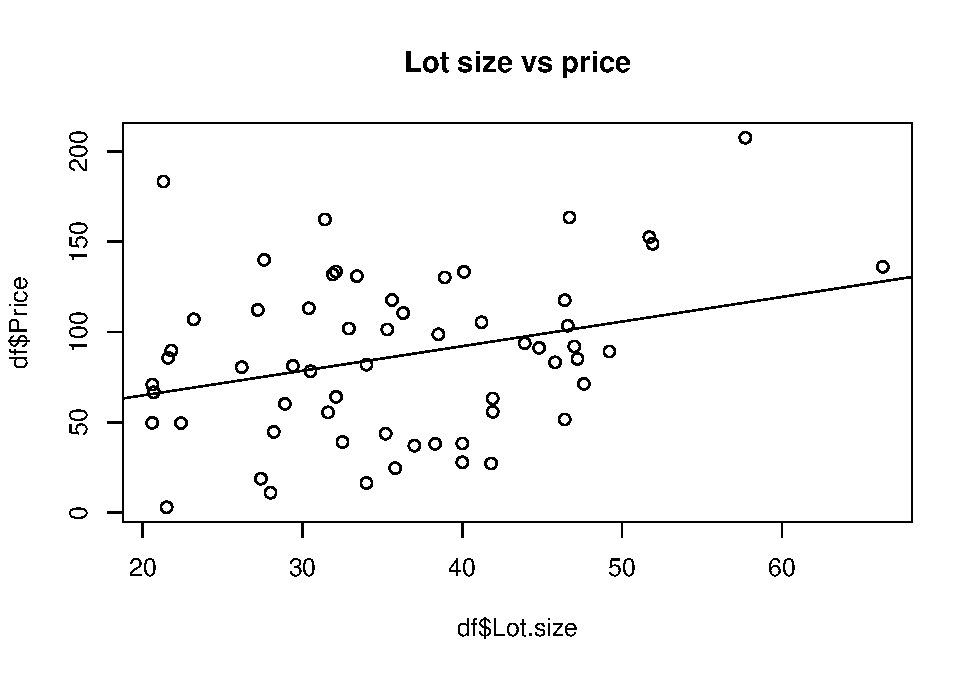
\includegraphics{103-hw5_files/figure-latex/unnamed-chunk-2-1.pdf}

\begin{center}\rule{0.5\linewidth}{0.5pt}\end{center}

\begin{enumerate}
\def\labelenumi{\arabic{enumi}.}
\setcounter{enumi}{1}
\tightlist
\item
  Construct a quadratic model.
\end{enumerate}

\begin{enumerate}
\def\labelenumi{\alph{enumi}.}
\tightlist
\item
  Is the P-value for the model significant? (Quote the P-value in your
  response.) P-value is 9.78e-15 so this is statistically significant
\item
  What is the P-value for the second-degree term? 4.8e-6
\item
  What is R2 for the model? What is? Which is more appropriate in
  evaluating the model? 2-adjustedRd.\\
  .5117, adjusted R-squared is .5009, I will use R-squared because we
  only have one predictor and adjusted is meaningless. Graph the Plot of
  Fitted Model and include it in your solutions. ***
\end{enumerate}

\begin{Shaded}
\begin{Highlighting}[]
\NormalTok{model2 <-}\StringTok{ }\KeywordTok{lm}\NormalTok{(}\DataTypeTok{formula=}\StringTok{`}\DataTypeTok{MPG Highway}\StringTok{`}\OperatorTok{~}\NormalTok{Horsepower}\OperatorTok{+}\KeywordTok{I}\NormalTok{(Horsepower}\OperatorTok{^}\DecValTok{2}\NormalTok{),}\DataTypeTok{data=}\NormalTok{cars)}
\KeywordTok{summary}\NormalTok{(model2)}
\end{Highlighting}
\end{Shaded}

\begin{verbatim}
## 
## Call:
## lm(formula = `MPG Highway` ~ Horsepower + I(Horsepower^2), data = cars)
## 
## Residuals:
##      Min       1Q   Median       3Q      Max 
## -10.3763  -2.1174  -0.0666   2.0292  13.7592 
## 
## Coefficients:
##                   Estimate Std. Error t value Pr(>|t|)    
## (Intercept)      5.020e+01  2.728e+00  18.400  < 2e-16 ***
## Horsepower      -2.252e-01  3.416e-02  -6.593 2.87e-09 ***
## I(Horsepower^2)  4.821e-04  9.906e-05   4.867 4.81e-06 ***
## ---
## Signif. codes:  0 '***' 0.001 '**' 0.01 '*' 0.05 '.' 0.1 ' ' 1
## 
## Residual standard error: 3.767 on 90 degrees of freedom
## Multiple R-squared:  0.5117, Adjusted R-squared:  0.5009 
## F-statistic: 47.16 on 2 and 90 DF,  p-value: 9.78e-15
\end{verbatim}

\begin{Shaded}
\begin{Highlighting}[]
\KeywordTok{plot}\NormalTok{(}\DataTypeTok{x=}\NormalTok{cars}\OperatorTok{$}\NormalTok{Horsepower,}\DataTypeTok{y=}\NormalTok{cars}\OperatorTok{$}\StringTok{`}\DataTypeTok{MPG Highway}\StringTok{`}\NormalTok{)}
\KeywordTok{lines}\NormalTok{(cars}\OperatorTok{$}\NormalTok{Horsepower, }\KeywordTok{fitted}\NormalTok{(model2), }\DataTypeTok{col=}\StringTok{"blue"}\NormalTok{)}
\end{Highlighting}
\end{Shaded}

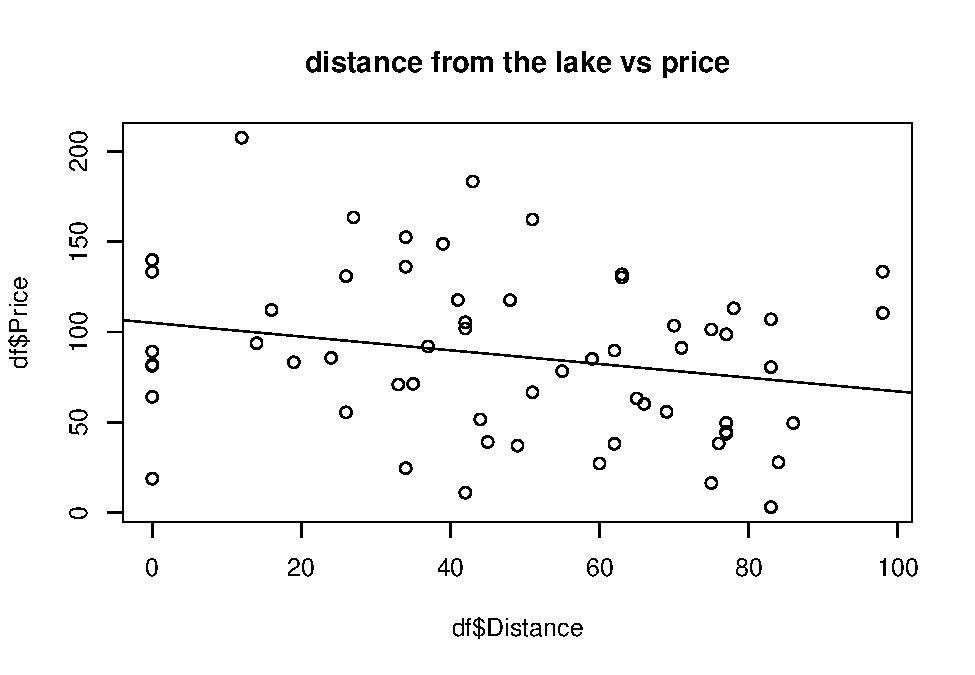
\includegraphics{103-hw5_files/figure-latex/unnamed-chunk-4-1.pdf}

\begin{center}\rule{0.5\linewidth}{0.5pt}\end{center}

\begin{enumerate}
\def\labelenumi{\arabic{enumi}.}
\setcounter{enumi}{2}
\tightlist
\item
  Try constructing higher order models until you are satisfied you have
  found the best polynomial model.
\end{enumerate}

\begin{enumerate}
\def\labelenumi{\alph{enumi}.}
\tightlist
\item
  Write out your final model or display the analysis window for it so I
  can see the model you settled on. The 4th degree polynomial funtion
  has the nighest adjusted R-squared
\item
  What is adjustedR2? .542
\item
  Include the Plot of Fitted Model and Residuals versus X output.
\item
  Predict the highway mileage of a car with 150 horsepower. Also
  construct 95\% confidence and prediction intervals for such a car. ***
\end{enumerate}

\begin{Shaded}
\begin{Highlighting}[]
\CommentTok{# model3 <- lm(formula=`MPG Highway`~Horsepower+I(Horsepower^2)+I(Horsepower^3),data=cars)}
\NormalTok{model4 <-}\StringTok{ }\KeywordTok{lm}\NormalTok{(}\DataTypeTok{formula=}\StringTok{`}\DataTypeTok{MPG Highway}\StringTok{`}\OperatorTok{~}\NormalTok{Horsepower}\OperatorTok{+}\KeywordTok{I}\NormalTok{(Horsepower}\OperatorTok{^}\DecValTok{2}\NormalTok{)}\OperatorTok{+}\KeywordTok{I}\NormalTok{(Horsepower}\OperatorTok{^}\DecValTok{3}\NormalTok{)}\OperatorTok{+}\KeywordTok{I}\NormalTok{(Horsepower}\OperatorTok{^}\DecValTok{4}\NormalTok{),}\DataTypeTok{data=}\NormalTok{cars)}
\CommentTok{# model5 <- lm(formula=`MPG Highway`~Horsepower+I(Horsepower^2)+I(Horsepower^3)+I(Horsepower^4)+I(Horsepower^5),data=cars)}
\CommentTok{# summary(model3)}
\KeywordTok{summary}\NormalTok{(model4)}
\end{Highlighting}
\end{Shaded}

\begin{verbatim}
## 
## Call:
## lm(formula = `MPG Highway` ~ Horsepower + I(Horsepower^2) + I(Horsepower^3) + 
##     I(Horsepower^4), data = cars)
## 
## Residuals:
##     Min      1Q  Median      3Q     Max 
## -9.1426 -1.6937  0.4241  1.6519 14.8495 
## 
## Coefficients:
##                   Estimate Std. Error t value Pr(>|t|)    
## (Intercept)      9.128e+01  1.707e+01   5.348 6.95e-07 ***
## Horsepower      -1.265e+00  4.723e-01  -2.678  0.00884 ** 
## I(Horsepower^2)  9.418e-03  4.598e-03   2.048  0.04352 *  
## I(Horsepower^3) -3.136e-05  1.869e-05  -1.677  0.09704 .  
## I(Horsepower^4)  3.848e-08  2.677e-08   1.438  0.15410    
## ---
## Signif. codes:  0 '***' 0.001 '**' 0.01 '*' 0.05 '.' 0.1 ' ' 1
## 
## Residual standard error: 3.608 on 88 degrees of freedom
## Multiple R-squared:  0.5619, Adjusted R-squared:  0.542 
## F-statistic: 28.22 on 4 and 88 DF,  p-value: 4.342e-15
\end{verbatim}

\begin{Shaded}
\begin{Highlighting}[]
\CommentTok{# summary(model5)}
\end{Highlighting}
\end{Shaded}

\begin{Shaded}
\begin{Highlighting}[]
\KeywordTok{plot}\NormalTok{(}\DataTypeTok{x=}\NormalTok{cars}\OperatorTok{$}\NormalTok{Horsepower,}\DataTypeTok{y=}\NormalTok{cars}\OperatorTok{$}\StringTok{`}\DataTypeTok{MPG Highway}\StringTok{`}\NormalTok{)}
\CommentTok{# lines(cars$Horsepower, fitted(model4), col="blue")}
\KeywordTok{lines}\NormalTok{(}\KeywordTok{spline}\NormalTok{(cars}\OperatorTok{$}\NormalTok{Horsepower, }\KeywordTok{fitted}\NormalTok{(model4)))}
\end{Highlighting}
\end{Shaded}

\includegraphics{103-hw5_files/figure-latex/unnamed-chunk-6-1.pdf}

\begin{Shaded}
\begin{Highlighting}[]
\KeywordTok{plot}\NormalTok{(model4}\OperatorTok{$}\NormalTok{fitted,model4}\OperatorTok{$}\NormalTok{resid)}
\end{Highlighting}
\end{Shaded}

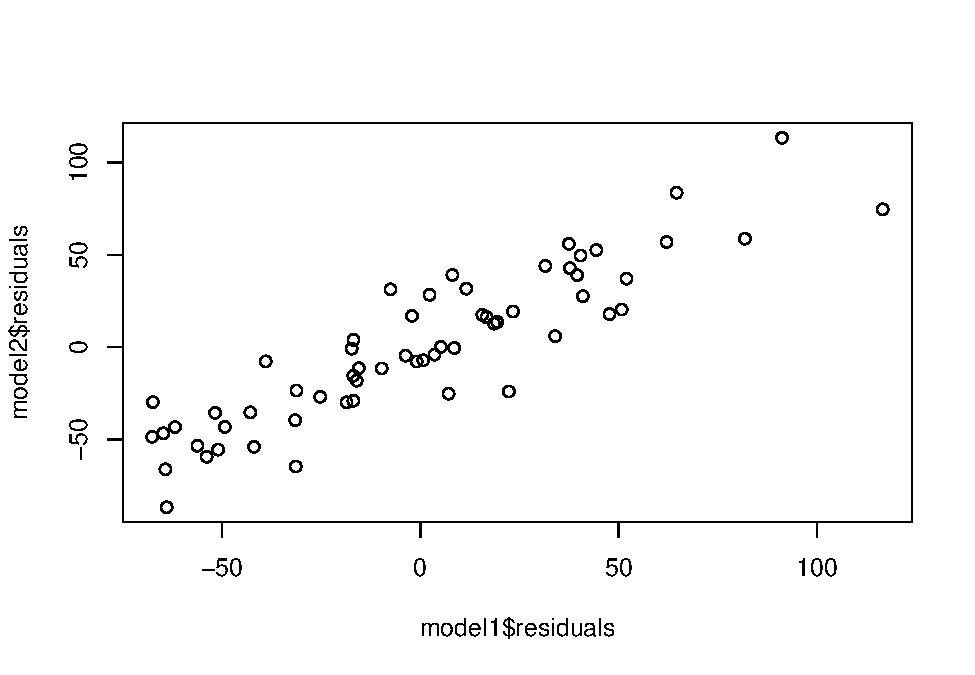
\includegraphics{103-hw5_files/figure-latex/unnamed-chunk-7-1.pdf}

\begin{Shaded}
\begin{Highlighting}[]
\NormalTok{test =}\StringTok{ }\KeywordTok{data.frame}\NormalTok{(}
  \DataTypeTok{Horsepower =} \DecValTok{150}
\NormalTok{)}
\KeywordTok{predict}\NormalTok{(model4,}\DataTypeTok{newdata=}\NormalTok{test,}\DataTypeTok{interval=}\StringTok{'confidence'}\NormalTok{)}
\end{Highlighting}
\end{Shaded}

\begin{verbatim}
##        fit      lwr      upr
## 1 27.12688 26.02405 28.22971
\end{verbatim}

\end{document}
